\documentclass[12pt, a4paper]{article}
\title{Эффект Поккельса (4.7.2)}
\author{Стеценко Георгий, Б02-312}
\date{}
% !TeX encoding = UTF-8

\usepackage{geometry}
\usepackage{amsmath, amsfonts, amssymb, amsthm} % стандартный набор AMS-пакетов для математ. текстов
\usepackage{mathtext}
\usepackage[utf8]{inputenc} % кодировка utf8
\usepackage[russian]{babel} % русский язык
\usepackage[pdftex,dvipsnames]{xcolor} % работа с цветами
\usepackage[pdftex]{graphicx} % графика (картинки)
\usepackage{tikz,pgfplots} % рисунки
\usepackage{indentfirst}
%\usepackage[labelfont=bf,labelsep=endash,skip=3pt]{caption} % подпись картинок
% \usepackage{fancyhdr,pageslts} % настройка колонтитулов
\usepackage{enumitem} % работа со списками
\usepackage{floatrow,multicol,multirow,longtable,hhline} % работа с таблицами
\usepackage{float,wrapfig} % плавающие объекты
\usepackage{tcolorbox} % рамка вокруг текста
%\usepackage[calc]{datetime2} % дата
\usepackage{bm} % жирное начертание в формулах
\usepackage{physics} % физический пакет
\DeclareMathAlphabet\mathbfcal{OMS}{cmsy}{b}{n}
\usepackage{pgfornament} % красивые рюшечки и вензеля
\usepackage{mdframed}
\usepackage{derivative}
\usepackage{mathrsfs} %EDS
\usepackage{soul} % strikethorugh
%\usepackage{boondox-cal}

% ----------------------------------------
% Настройка шрифта

% Просто закооментируйте следующую строчку, если не работает. Будет другой шрифт, правда :(
% \usepackage{pscyr}

% ----------------------------------------
% Стилевые настройки

\usepackage{boldline} % жирная линия после таблиц (чтобы не было ошибок, этот пакет должен подключаться именно тут!)
\floatsetup[table]{style=Plaintop,floatrowsep=qquad} % настройка оформления таблиц
\setlist[enumerate,itemize]{leftmargin=5mm,itemindent=10mm,itemsep=0mm,
listparindent=0em,labelsep=2mm,topsep=2mm,labelwidth=4mm} % настройки списков

\setlength{\columnsep}{0.5cm} % расстояние между колонками
\setlength{\parskip}{1pt} % расстояние до текста от колонтитула

%\usepackage{titlesec} % управление оформлением section
%\renewcommand{\thesection}{\Roman{section}}
%\titleformat{\section}[block]{\bfseries\large}{\thesection.}{5pt}{}

% ----------------------------------------
% Настройки полей
\geometry{
  left=10mm,
  top=10mm,
  right=10mm,
  bottom=15mm,
  marginparsep=0mm,
  marginparwidth=0mm,
  headheight=0pt,
  headsep=0pt,
footskip=20pt}

% ----------------------------------------
% Настройки колонтитулов и нумерации страниц
\pagenumbering{arabic}



\newcounter{ntask}
\setcounter{ntask}{0}


\newcommand{\arsh}{\mathrm{arsh} \,\,}
\newcommand{\arch}{\mathrm{arch} \,\,}
\newcommand{\arth}{\mathrm{arth} \,\,}
\newcommand{\arcth}{\mathrm{arcth} \,\,}
\renewcommand{\Re}{\operatorname{Re} \,}
\newcommand{\EDS}{\mathscr{E}}
\newcommand{\diffract}[1]{\frac{\mathrm{d}#1}{\mathrm{d}t}}


\newcommand{\mim}{~\mathrm{mm}}

\addto\captionsrussian{\def\refname{Источники}}

\begin{document}
\maketitle

\textbf{Цель:} исследовать интерференцию рассеянного света, прошедшего
кристалл; наблюдать изменение характера поляризации света при наложении на
кристалл электрического поля.

\textbf{Оборудование:} гелий-неоновый лазер, поляризатор, кристалл ниобата
лития, матовая пластинка, экран, источник высоковольтного переменного и
постоянного напряжения, фотодиод, осциллограф, линейка.

\section{Теоретические сведения}
Эффект Поккельса -- изменение показателя преломления света в кристалле под
действием электрического поля.

Рассмотрим кристалл ниобата лития $\text{LiNbO}_3$ с цетральноосевой симметрией
вдоль оси $Z$. Для световой волны с $\mathbf{E}$ перпендикулярно $Z$ показатель
преломления будет $n_o$, а для волны с $\mathbf{E}$ вдоль $Z$ -- $n_e$. В
случае, когда луч света идёт под углом $\theta$ к оси, есть два значение
показателя преломления $n_1$ и $n_2$: $n_1 = n_o$ для волны с $\mathbf{E}$
перпендикулярным плоскости $(\mathbf{k},\mathbf{Z})$ (обыкновенная волна) и
$n_2$ для волны с $\mathbf{E}$ в этой плоскости (необыкновенная волна). В
последнем случае
\begin{equation}
    \dfrac{1}{n_2^2}=\dfrac{\cos^2 \theta}{n_0^2}+\dfrac{\sin^2 \theta}{n_e^2}.
\end{equation}

\begin{figure}[h]
    \center{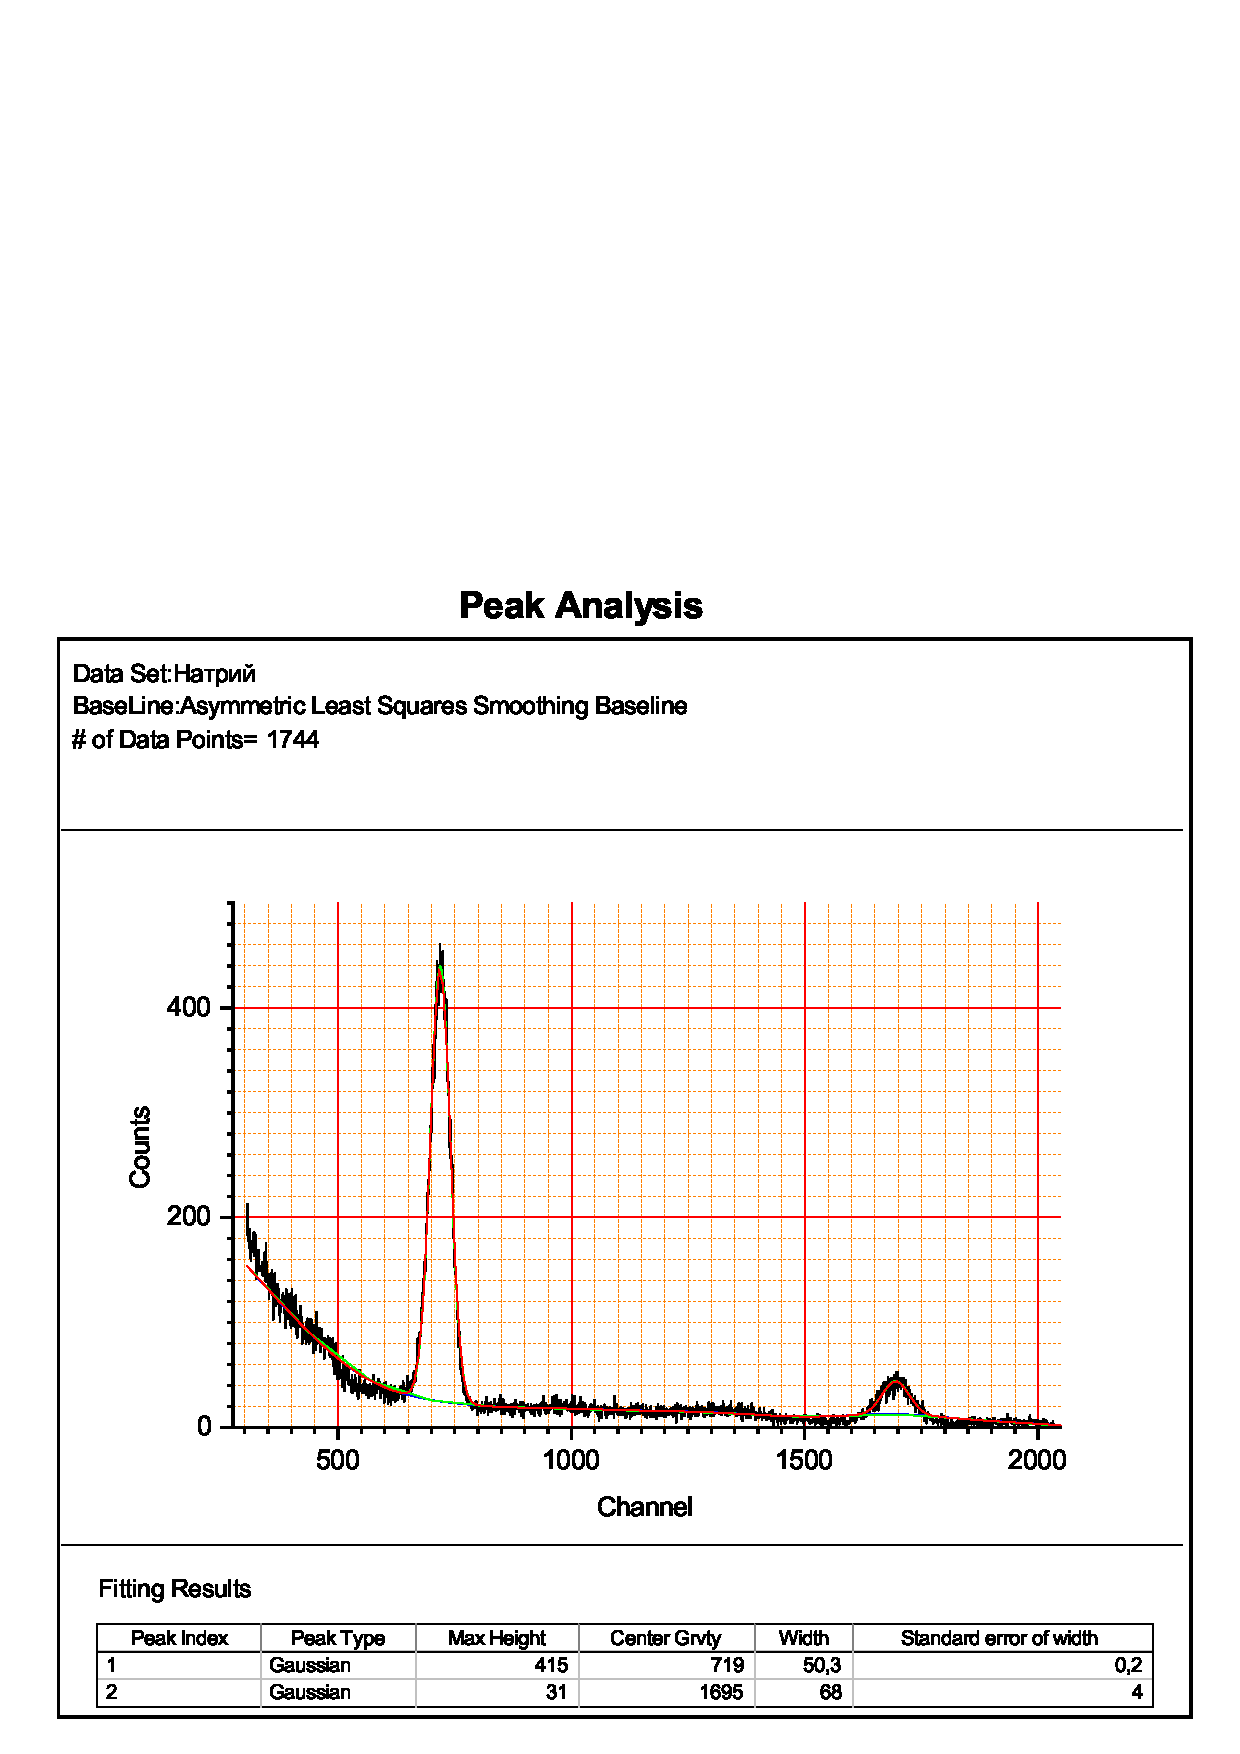
\includegraphics[scale=0.5]{pics/1.jpg}}
    \caption{\centering Оптическая часть экспериментальной установки}
    \label{fig:setup}
\end{figure}

Если перед кристаллом, помещённым между поляроидами, расположить линзу или
матовую пластинку, то на экране за поляроидом мы увидим тёмные концентрические
окружности -- результат интерференции обыкновенной и необыкновенной волн. При
повороте выходного поляроида на $90^\circ$ картина меняется с позитива на
негатив (на месте светлых пятен появляются тёмные и наоборот). В случае, когда
разрешённое направление анализатора перпендикулярно поляризации лазерного
излучения, радиус тёмного кольца с номером $m$ равен
\begin{equation}
    r_m^2 = \dfrac{\lambda}{l} \dfrac{(n_oL)^2}{n_0 - n_e}m,
    \label{eq:radius}
\end{equation}

\begin{figure}[h]
    \center{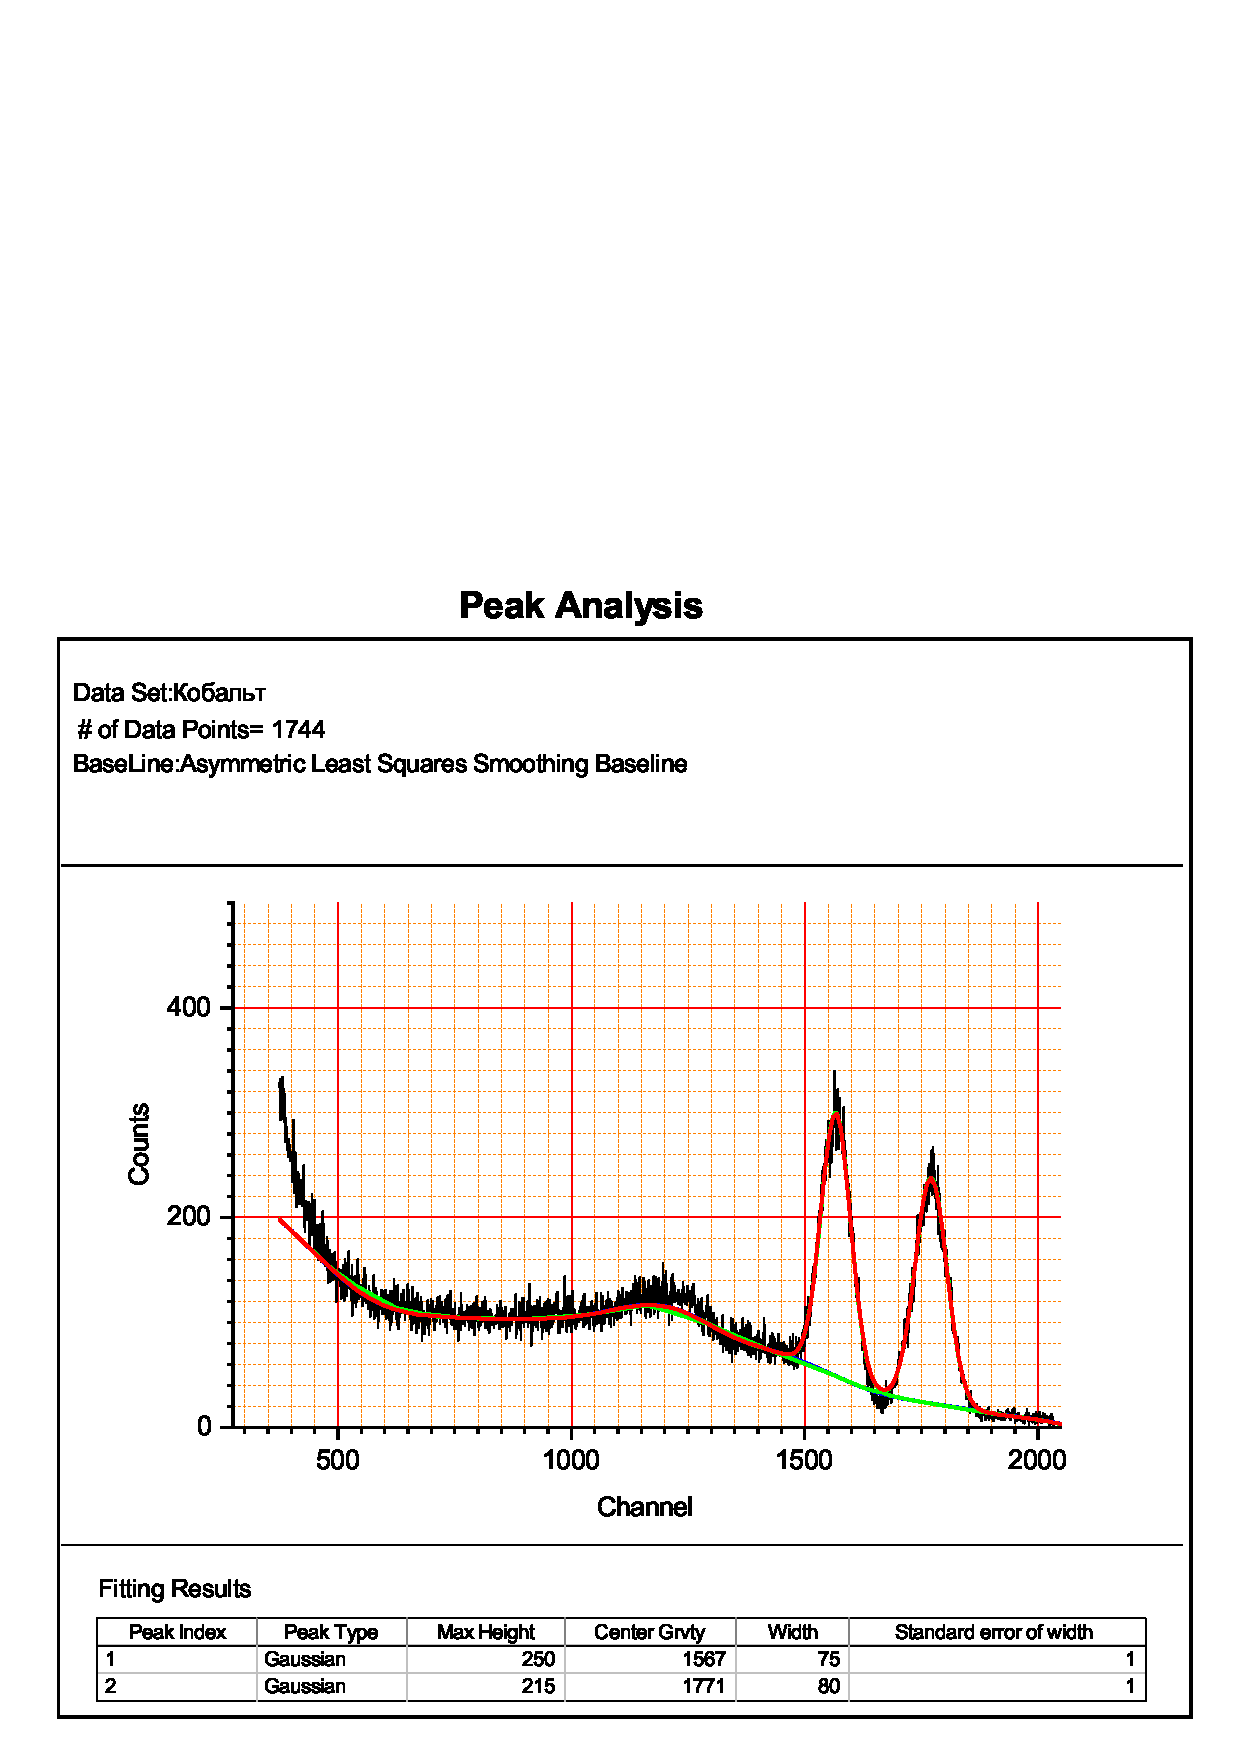
\includegraphics[scale=0.5]{pics/2.jpg}}
    \caption{\centering Экспериментальная установка}
    \label{fig:image1}
\end{figure}

где $L$ -- расстояние от центра кристалла до экрана, $l$ -- длина кристалла.

Теперь поместим кристалл в постоянное электрическое поле $E_{\text{эл}}$,
направленное вдоль оси $X$, перпендикулярной $Z$. Показатель преломления для
луча, распространяющего вдоль $Z$, всегда $n_o$. В плоскости $(X,Y)$ возникают
два главных направления под углами $45^\circ$ к $X$ и $Y$ с показателями
преломления $n_0 - \Delta n$ и $n_o + \Delta n$ (быстрая и медленная ось),
причём $\Delta n = A E_{\text{эл}}$. Для поляризованного вертикально света и
анализатора, пропускающего горизонтальную поляризацию, на выходе интенсивность
на выходе будет иметь вид
\begin{equation}
    I_{\text{вых}} = I_0 \sin^2 \left(\dfrac{\pi}{2} \dfrac{U}{U_{\lambda/2}} \right),
\end{equation}
где $\displaystyle U_{\lambda/2} = \frac{\lambda}{4A}\frac{d}{l}$ -- \textit{полуволновое напряжение}, $d$ -- поперечный размер кристалла.  При напряжении $U = E_{\text{эл}}d$ равном полуволновому сдвиг фаз между двумя волнами равен $\pi$, а интенсивность света на выходе максимальна.

На Рис. 2 представлена схема всей установки (оптическая часть изорбажена на
Рис. 1). Свет лазера, проходя через сквозь пластину, рассеивается и падает на
двоякопреломляющий кристалл. На экране за поляроидом видна интерференционная
картина. Убрав рассеивающую пластину и подавая на кристалл постоянное
напряжение, можно величиной напряжения влиять на поляризацию луча, вышедшего из
кристалла. Заменив экран фотодиодом и подав на кристалл переменное напряжение,
можно исследовать поляризацию с помощью осциллографа.

\section{Методика измерений и результаты}
\subsection{Измерение двулучепреломления без подачи напряжения}
Соберем схему установку рис. \ref{fig:setup}. Наблюдаем интерференционную
картину на экране: концентрические кольца, рассечённые тёмным <<мальтийским
крестом>>.

\begin{table}[h!]
    \centering
    \caption{Результаты измерений радиусов колец}
    \begin{tabular}{|c|c|c|c|c|c|c|}
        \hline
        Номер кольца     & 1    & 2    & 3    & 4    & 5    & 6    \\
        \hline
        $R_1$            & 31   & 45   & 53   & 62   & 70   & 78   \\
        \hline
        $R_2$            & 31   & 44   & 53   & 61   & 72   & 77   \\
        \hline
        $R_3$            & 30   & 43   & 54   & 62   & ---  & ---  \\
        \hline
        $R_4$            & 33   & 43   & 55   & 63   & ---  & ---  \\
        \hline
        \textbf{Среднее} & 31.3 & 43.8 & 53.8 & 62.0 & 71.0 & 77.5 \\
        \hline
    \end{tabular}
\end{table}

Построим график зависимости $R^2$ от номера кольца $m$ (Рис. \ref{fig:graph1}).
\begin{figure}[H]
    \centering
    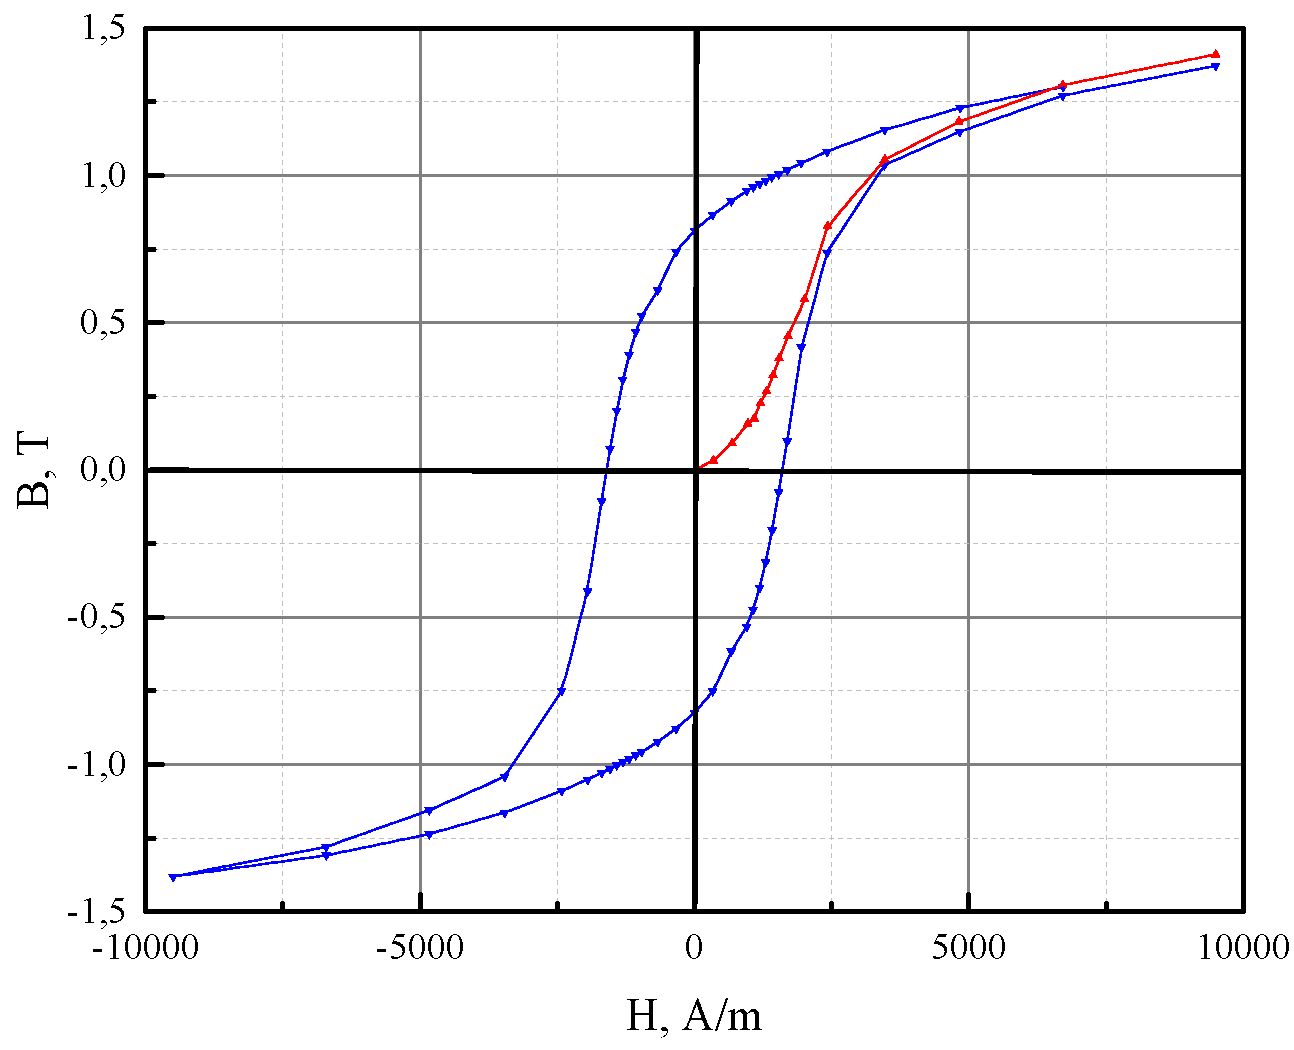
\includegraphics[width=0.9\linewidth]{pics/plot.png}
    \caption{Зависимость $R^2$ от номера кольца $m$}
    \label{fig:graph1}
\end{figure}
Пользуясь формулой \eqref{eq:radius}, определим двулучепреломление кристалла.
$\lambda = 630~\mathrm{nm}$, $l = 26\mim$, $n_0 = 2.29$, $L = 84~\mathrm{cm}$.

$$n_{o}-n_{e} = \dfrac{\lambda}{l} \dfrac{(n_oL)^2}{k} = 0.088 \pm 0.004$$
что соотвествует табличному значению.

\subsection{Определение полуволнового напряжения}
В данном пункте работы была убрана матовая пластинка, и был проделан опыт с
увеличением напряжения на кристалле и измерением максимумов и минимумов
интенсивности. Полученные результаты приведены в таблице 2 (считаем абсолютную
погрешность равной половине деления).

\begin{table}[h]
    \begin{tabular}{|l|l|l|}
        \hline
        $U_{\lambda/2}$ & $U_{\lambda}$ & $U_{3\lambda/2}$ \\ \hline
        480             & 960           & 1440             \\ \hline
    \end{tabular}
    \caption{Результаты измерений полуволнового напряжения}
\end{table}

Проверим также, что при выставлении напряжения $U_{\lambda/4}$ получается
круговая поляризация (интенсивность не меняется при вращении анализатора).

Также подадим переменное напряжение на кристалл, и пронаблюдаем фигуру Лиссажу.
Она представляет из себя синусоиду, экстремумы которой соответсвуют
напряжениям, кратным полуволновым.

\section{Вывод}
В работе с помощью интерференционной картины было определено двулучепреломления
ниобата лития, которое с хорошей точностью сошлось с табличным значением. Также
был исследован эффект Поккельса и определено полуволновое напряжение помощью
наблюдения за изменением интенсивности, также полученное значение было
проверено с помощью следующего факта: при напряжении $U_{\lambda/4}$ получается
круговая поляризация.

\end{document}